A very high-level overview of the topic is given here.

\lipsum[1]

\section{circRNAs}
This section describes what circRNAs are, how they are formed, and what their functions are.
It also gives insights into the current state of research.

\subsection{Biogenesis}
This subsection describes how circRNAs are formed.

\begin{figure}[H]
    \centering
    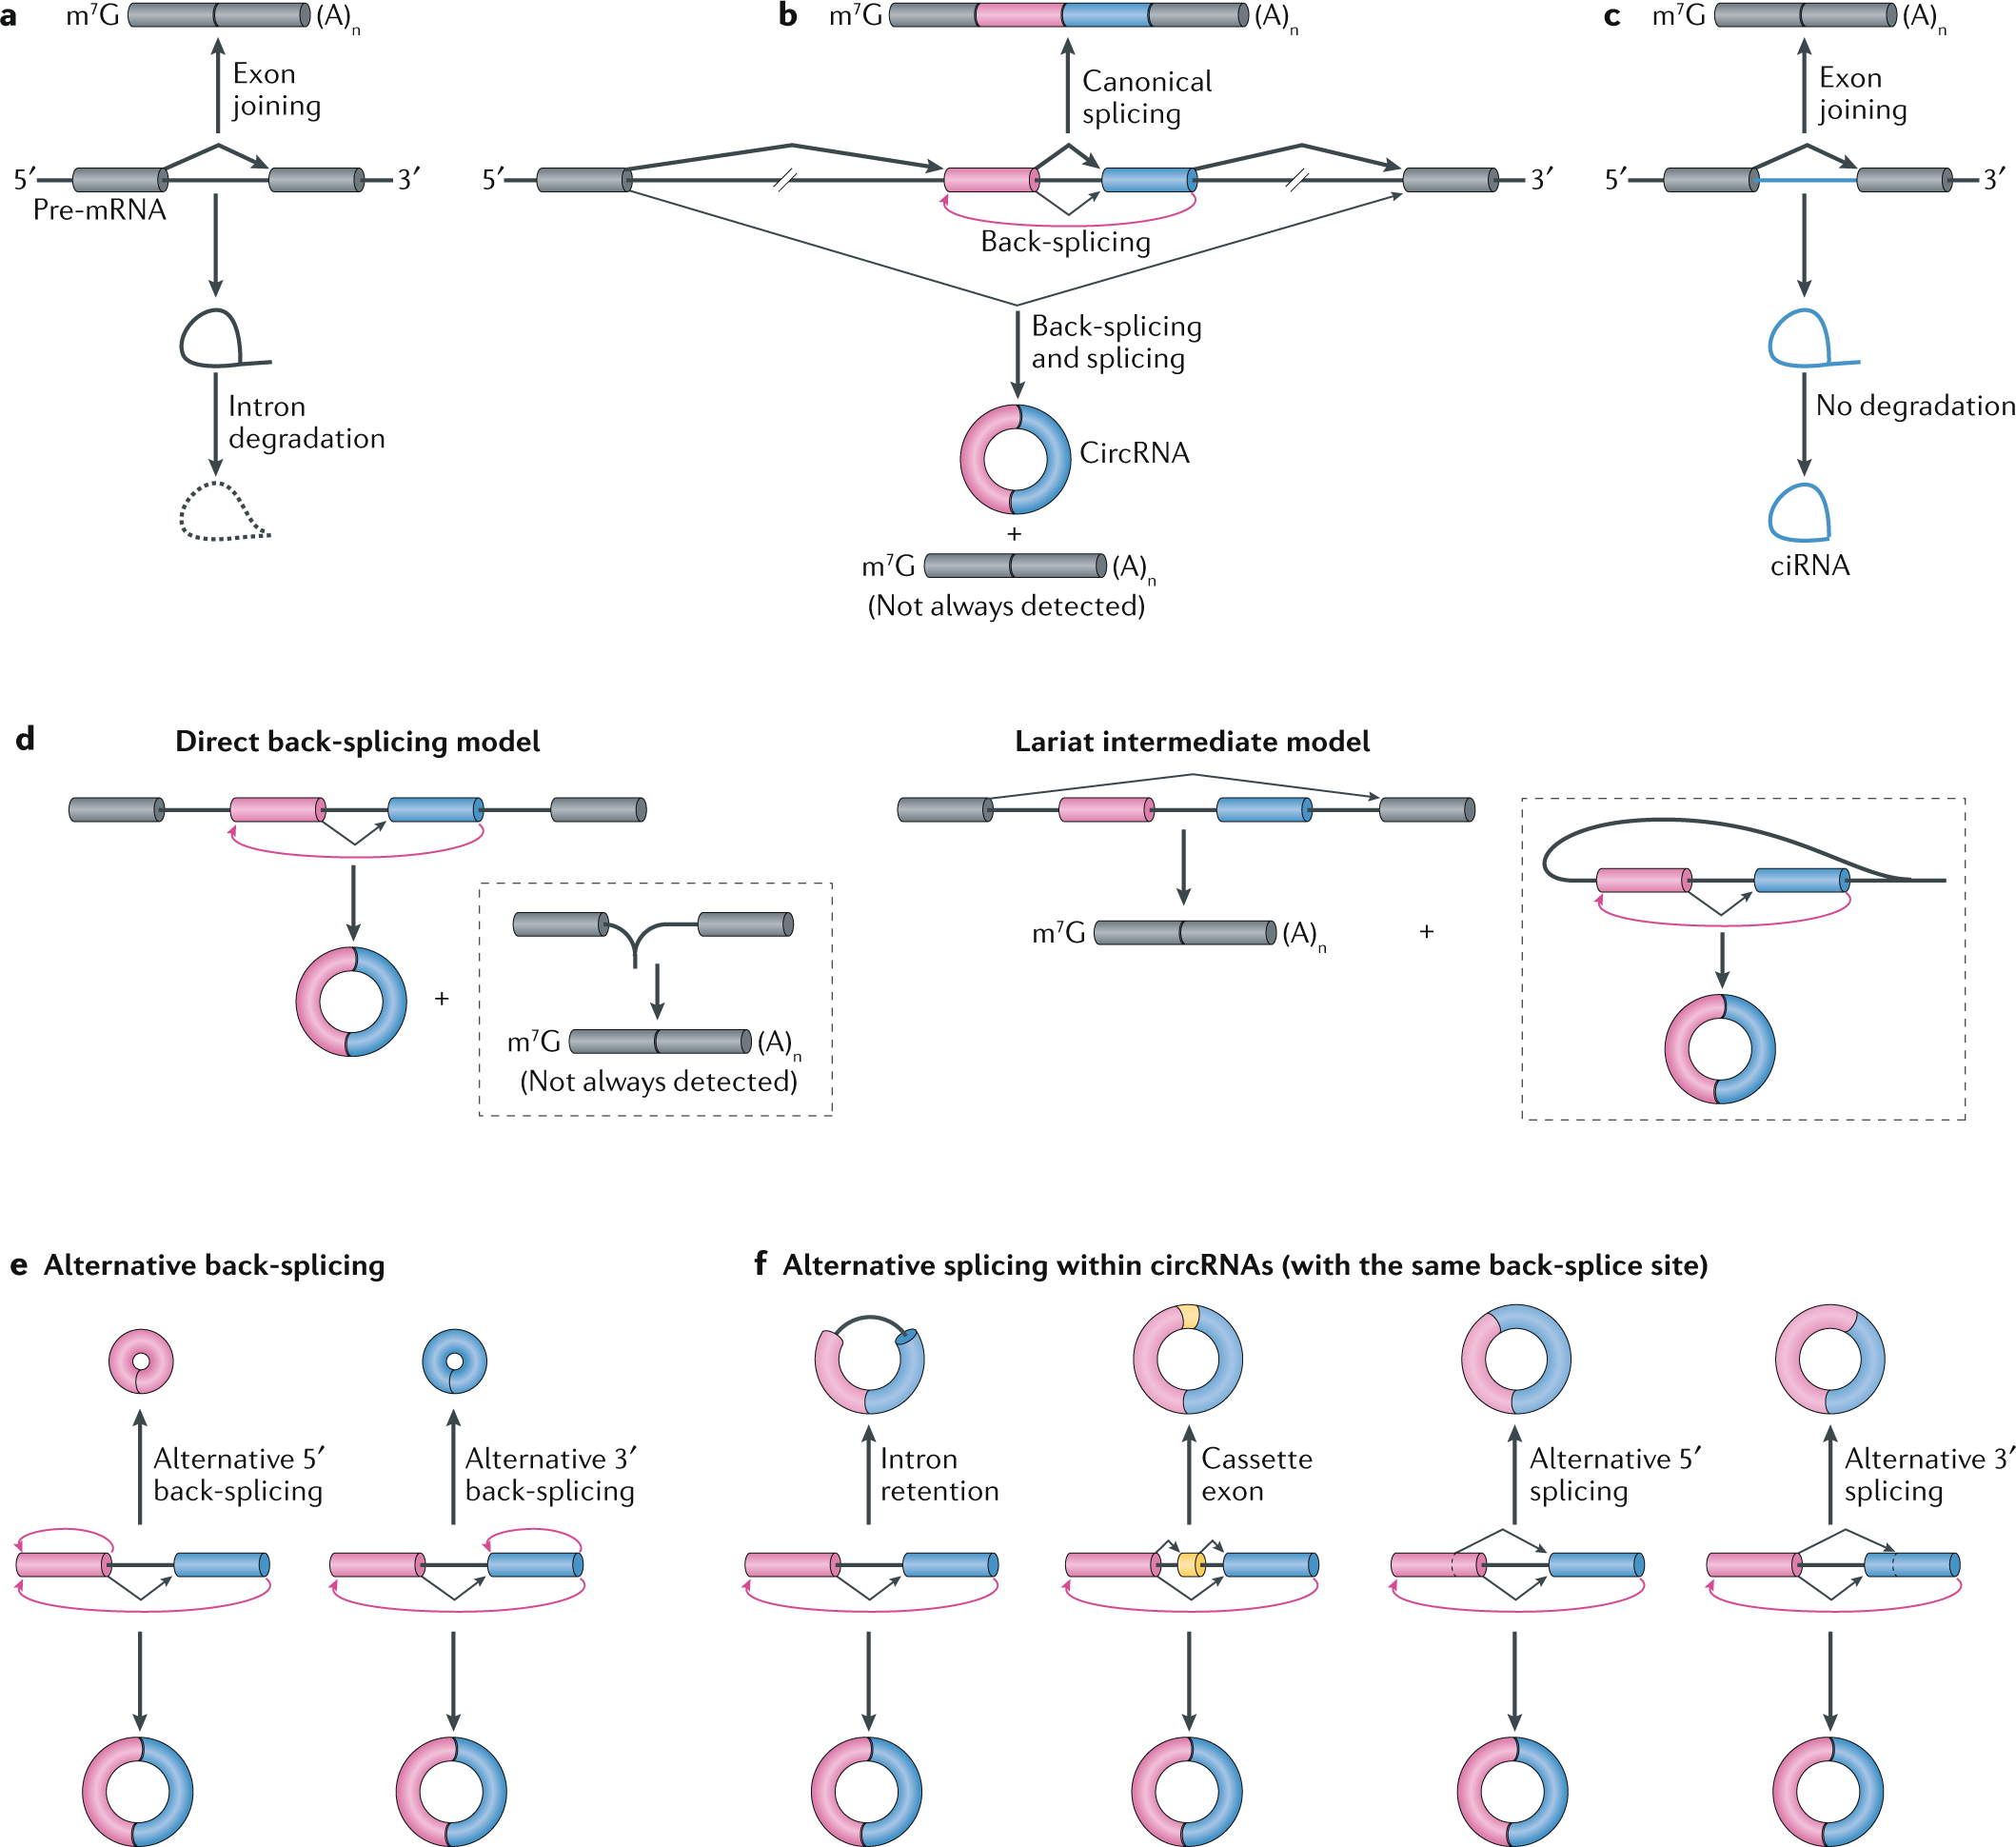
\includegraphics[width=\textwidth]{chapters/background/figures/circRNA-splicing.png}
    \caption{Splicing of circRNAs}
    \label{fig:circRNA_splicing}
\end{figure}

\subsection{Functions}
This subsection describes what functions circRNAs have.

\subsubsection{miRNA sponges}
This subsubsection describes how circRNAs can act as miRNA sponges.

\subsubsection{Protein binding}
This subsubsection describes how circRNAs can bind to proteins.

\subsubsection{Protein coding}
This subsubsection describes how circRNAs can code for proteins.

\subsection{Existing research}
This subsection describes the current state of research on circRNAs.

\section{totalRNA sequencing}
This subsection describes the sequencing method used to identify circRNAs.

\lipsum[2]

\section{Breast cancer}
This section describes what breast cancer is, how it is diagnosed, and what the current treatment options are.
It also gives insights into the current state of research.

\lipsum[3]

\section{Estrogen signaling}
This section describes what estrogen is, how it affects breast cancer, and what the current treatment options are.
It also gives insights into the current state of research.

\lipsum[4]

\section{Related work}
This section describes related work on circRNAs, breast cancer, and estrogen signaling.

\subsection{circRNA-sponging pipeline}
This subsection describes a pipeline for identifying circRNA sponges.